% TEMPLATE for Usenix papers, specifically to meet requirements of
%  USENIX '05
% originally a template for producing IEEE-format articles using LaTeX.
%   written by Matthew Ward, CS Department, Worcester Polytechnic Institute.
% adapted by David Beazley for his excellent SWIG paper in Proceedings,
%   Tcl 96
% turned into a smartass generic template by De Clarke, with thanks to
%   both the above pioneers
% use at your own risk.  Complaints to /dev/null.
% make it two column with no page numbering, default is 10 point

% Munged by Fred Douglis <douglis@research.att.com> 10/97 to separate
% the .sty file from the LaTeX source template, so that people can
% more easily include the .sty file into an existing document.  Also
% changed to more closely follow the style guidelines as represented
% by the Word sample file. 

% Note that since 2010, USENIX does not require endnotes. If you want
% foot of page notes, don't include the endnotes package in the 
% usepackage command, below.

% This version uses the latex2e styles, not the very ancient 2.09 stuff.
\documentclass[letterpaper,twocolumn,10pt]{article}
\usepackage{usenix,epsfig}
\usepackage{times}  
\usepackage{epsfig}
\usepackage[TABBOTCAP]{subfigure}
\usepackage{tabularx}
\usepackage{graphicx} 
\usepackage{color}
\usepackage{xspace}
\usepackage{thumbpdf}
\usepackage{listings}
\usepackage{verbatim}
\usepackage{hyperref}
\usepackage{booktabs}
\usepackage{colortbl}
\usepackage[inline]{aplcomments}
\usepackage{inconsolata}
\usepackage{paralist}
\usepackage{xspace}
\usepackage{listings}
\lstset{
  basicstyle=\ttfamily,
  mathescape
}

\newcommenter{ak}{1.0,1.0,0.3}
\newcommenter{ac}{0.4,1.0,1.0}
\newcommand{\pktlanguage}{Domino\xspace}
\begin{document}

%don't want date printed
\date{}

%make title bold and 14 pt font (Latex default is non-bold, 16 pt)
%\title{\Large \bf Wonderful : A Terrific Application and Fascinating Paper}
\title{}

%for single author (just remove % characters)
\author{}
% copy the following lines to add more authors
% \and
% {\rm Name}\\
%Name Institution
%} % end author

\maketitle

% Use the following at camera-ready time to suppress page numbers.
% Comment it out when you first submit the paper for review.
%\thispagestyle{empty}

\subsection*{Abstract}
Data-plane algorithms execute on every packet traversing a network switch; they
encompass many schemes for congestion control, scheduling, network measurement,
active-queue management, security, and load balancing. Because these algorithms
are implemented in hardware today, they cannot be changed after being built. To
address this problem, recent work has proposed designs for programmable
line-rate switches.  However, these chips have only been used to program
stateless data-plane tasks, such as packet forwarding and access control. By
contrast, many data-plane algorithms create and modify algorithmic state on a
as part of their packet processing.

This paper presents \pktlanguage, a C-like imperative language to express
data-plane algorithms. \pktlanguage introduces the notion of a {\em packet
transaction}, defined as a sequential code block that is atomic and isolated
from other such code blocks.  The \pktlanguage compiler compiles \pktlanguage
code to \absmachine, a family of machine models based on emerging
programmable switch chipsets. We evaluate \pktlanguage by first designing
concrete \absmachine machines that support a variety of data-plane algorithms
with modest die area overhead. We then show how \pktlanguage simplifies
programming them, relative to current languages for programmable switches.

\section{Introduction}
\label{s:intro}

Data-plane algorithms~\cite{cestan} are algorithms that are implemented within
a network switch. These algorithms process every data packet that passes
through the switch, transforming the packet and often also some state stored on
the switch.  Examples of such algorithms include congestion-control that uses
feedback from switches~\cite{xcp, rcp, pdq, dctcp}, active queue
management~\cite{codel}, network measurement~\cite{opensketch, bitmap_george,
elephant_george}, and load-balanced routing in the data plane~\cite{conga}.

Because data-plane algorithms process every packet, an important implementation
requirement is the ability to process packets at line rate.  Consequently,
these algorithms are primarily implemented using dedicated hardware. However,
hardware designs are rigid, making it difficult to experiment with new
algorithms.

This rigidity affects network switch vendors that build network
equipment~\cite{cisco_nexus, dell_force10, arista_7050} based on
merchant-silicon switching chips~\cite{trident, tomahawk, mellanox}, network
operators using such chips within private networks~\cite{google,facebook,vl2},
and researchers developing new switch algorithms~\cite{xcp, codel, d3, detail,
pdq}. Today, the only way to implement a new data-plane algorithm at line rate
is to expressly build hardware for it---a time-consuming and resource-intensive
process.

Programmable switching chips~\cite{flexpipe, xpliant, rmt}, which are
competitive with state of the art fixed-function chipsets~\cite{trident,
tomahawk, mellanox}, have emerged as an alternative.  These chips allow network
programmers to express their algorithms using primitives provided by the chip.
Programming these chips has become more user-friendly over time. Initial
attempts used proprietary SDKs such as those from XPliant~\cite{xpliant_sdk,
xpliant_sdk2} and Intel~\cite{intel_sdk} that were closely tied to the
underlying hardware.  Over time, languages such as P4~\cite{p4, p4spec} have
raised the level of abstraction by providing a language that seeks to be
protocol and target independent.

While P4 considerably eases data-plane programming~\cite{dc_p4} relative to
fixed SDKs, it currently expects the programmer to understand the underlying
hardware. For instance, P4 requires the programmer to specify the
sequence of match-action tables that every packet goes through, requiring
programmers to understand hardware details such as pipeline stages and tables.
Network programmers would prefer more familiar abstractions such as
packet-processing languages for software routers~\cite{click} and network
processors~\cite{packetc, nova} that are modeled after higher level languages
such as C.

To this end, this paper presents \pktlanguage, a new DSL for expressing data-plane
algorithms. \pktlanguage is an imperative language based on C that allows
programmers to express data-plane algorithms using {\em packet transactions}
(\S\ref{s:transactions}).  Packet transactions provide the abstraction of a
sequential block of code that runs to completion on each packet before
executing on the next packet. This is a convenient programming model, since it
allows the programmer to focus on the operations needed for each packet without
worrying about other packets concurrently being processed by the switch
pipeline or hardware details such as pipeline stages.

We have implemented a compiler for \pktlanguage that compiles \pktlanguage
packet transactions and generates code for a family of abstract machines called
\absmachine~(\S\ref{s:absmachine}) (for Protocol-Independent Switch
Architecture). \absmachine generalizes recent work on the Reconfigurable Match
Table~\cite{rmt} model and captures essential features of programmable switch
architectures~\cite{rmt, xpliant, flexpipe}.

In addition, \absmachine introduces the concept of {\em atoms} to represent
atomic computations provided natively by a \absmachine machine much like
load-link/store-conditional, compare-and-exchange, and packed-multiply-and-add
on x86 machines today~\cite{x86_manual}.  Atoms provide the underlying atomic
hardware operations required to implement the programmer's view of packet
transactions, similar to how an atomic test-and-set is used to implement an
atomic increment.
%A template of the atoms available in a \absmachine machine is provided to the
%\pktlanguage compiler for code generation.

The \pktlanguage compiler guarantees deterministic performance for packet
transactions: all packet transactions that are implementable on a given switch
architecture will be executed at the switch's line rate, or they will be
rejected by the compiler if the atoms provided by a \absmachine machine cannot
implement the programmer-supplied transaction.

To evaluate the usefulness of \pktlanguage, we use \pktlanguage to express
several data-plane algorithms~(\S\ref{s:eval}) such as flowlet
switching~\cite{flowlets}, data-plane bloom filters~\cite{bloom}, heavy-hitter
detection~\cite{opensketch}, and CONGA~\cite{conga}.  The \pktlanguage compiler
determines if each algorithm can run at line rate on several different
\absmachine machines that differ in the atoms they
provide~(Table~\ref{table:eval}).
%We
%place \pktlanguage in the context of related work~(\S\ref{s:related}) and
%conclude by outlining several areas for future work~(\S\ref{s:future}).

\section{Context and system overview}

We present an abstract machine, \textit{\absmachine} that captures several
important features of programmable switch architectures~(\S\ref{ss:abstract})
with deterministic performance. \absmachine is our compiler target throughout
the paper.

\subsection{\absmachine: An abstract machine for programmable switches}
\begin{figure*}[!t]
  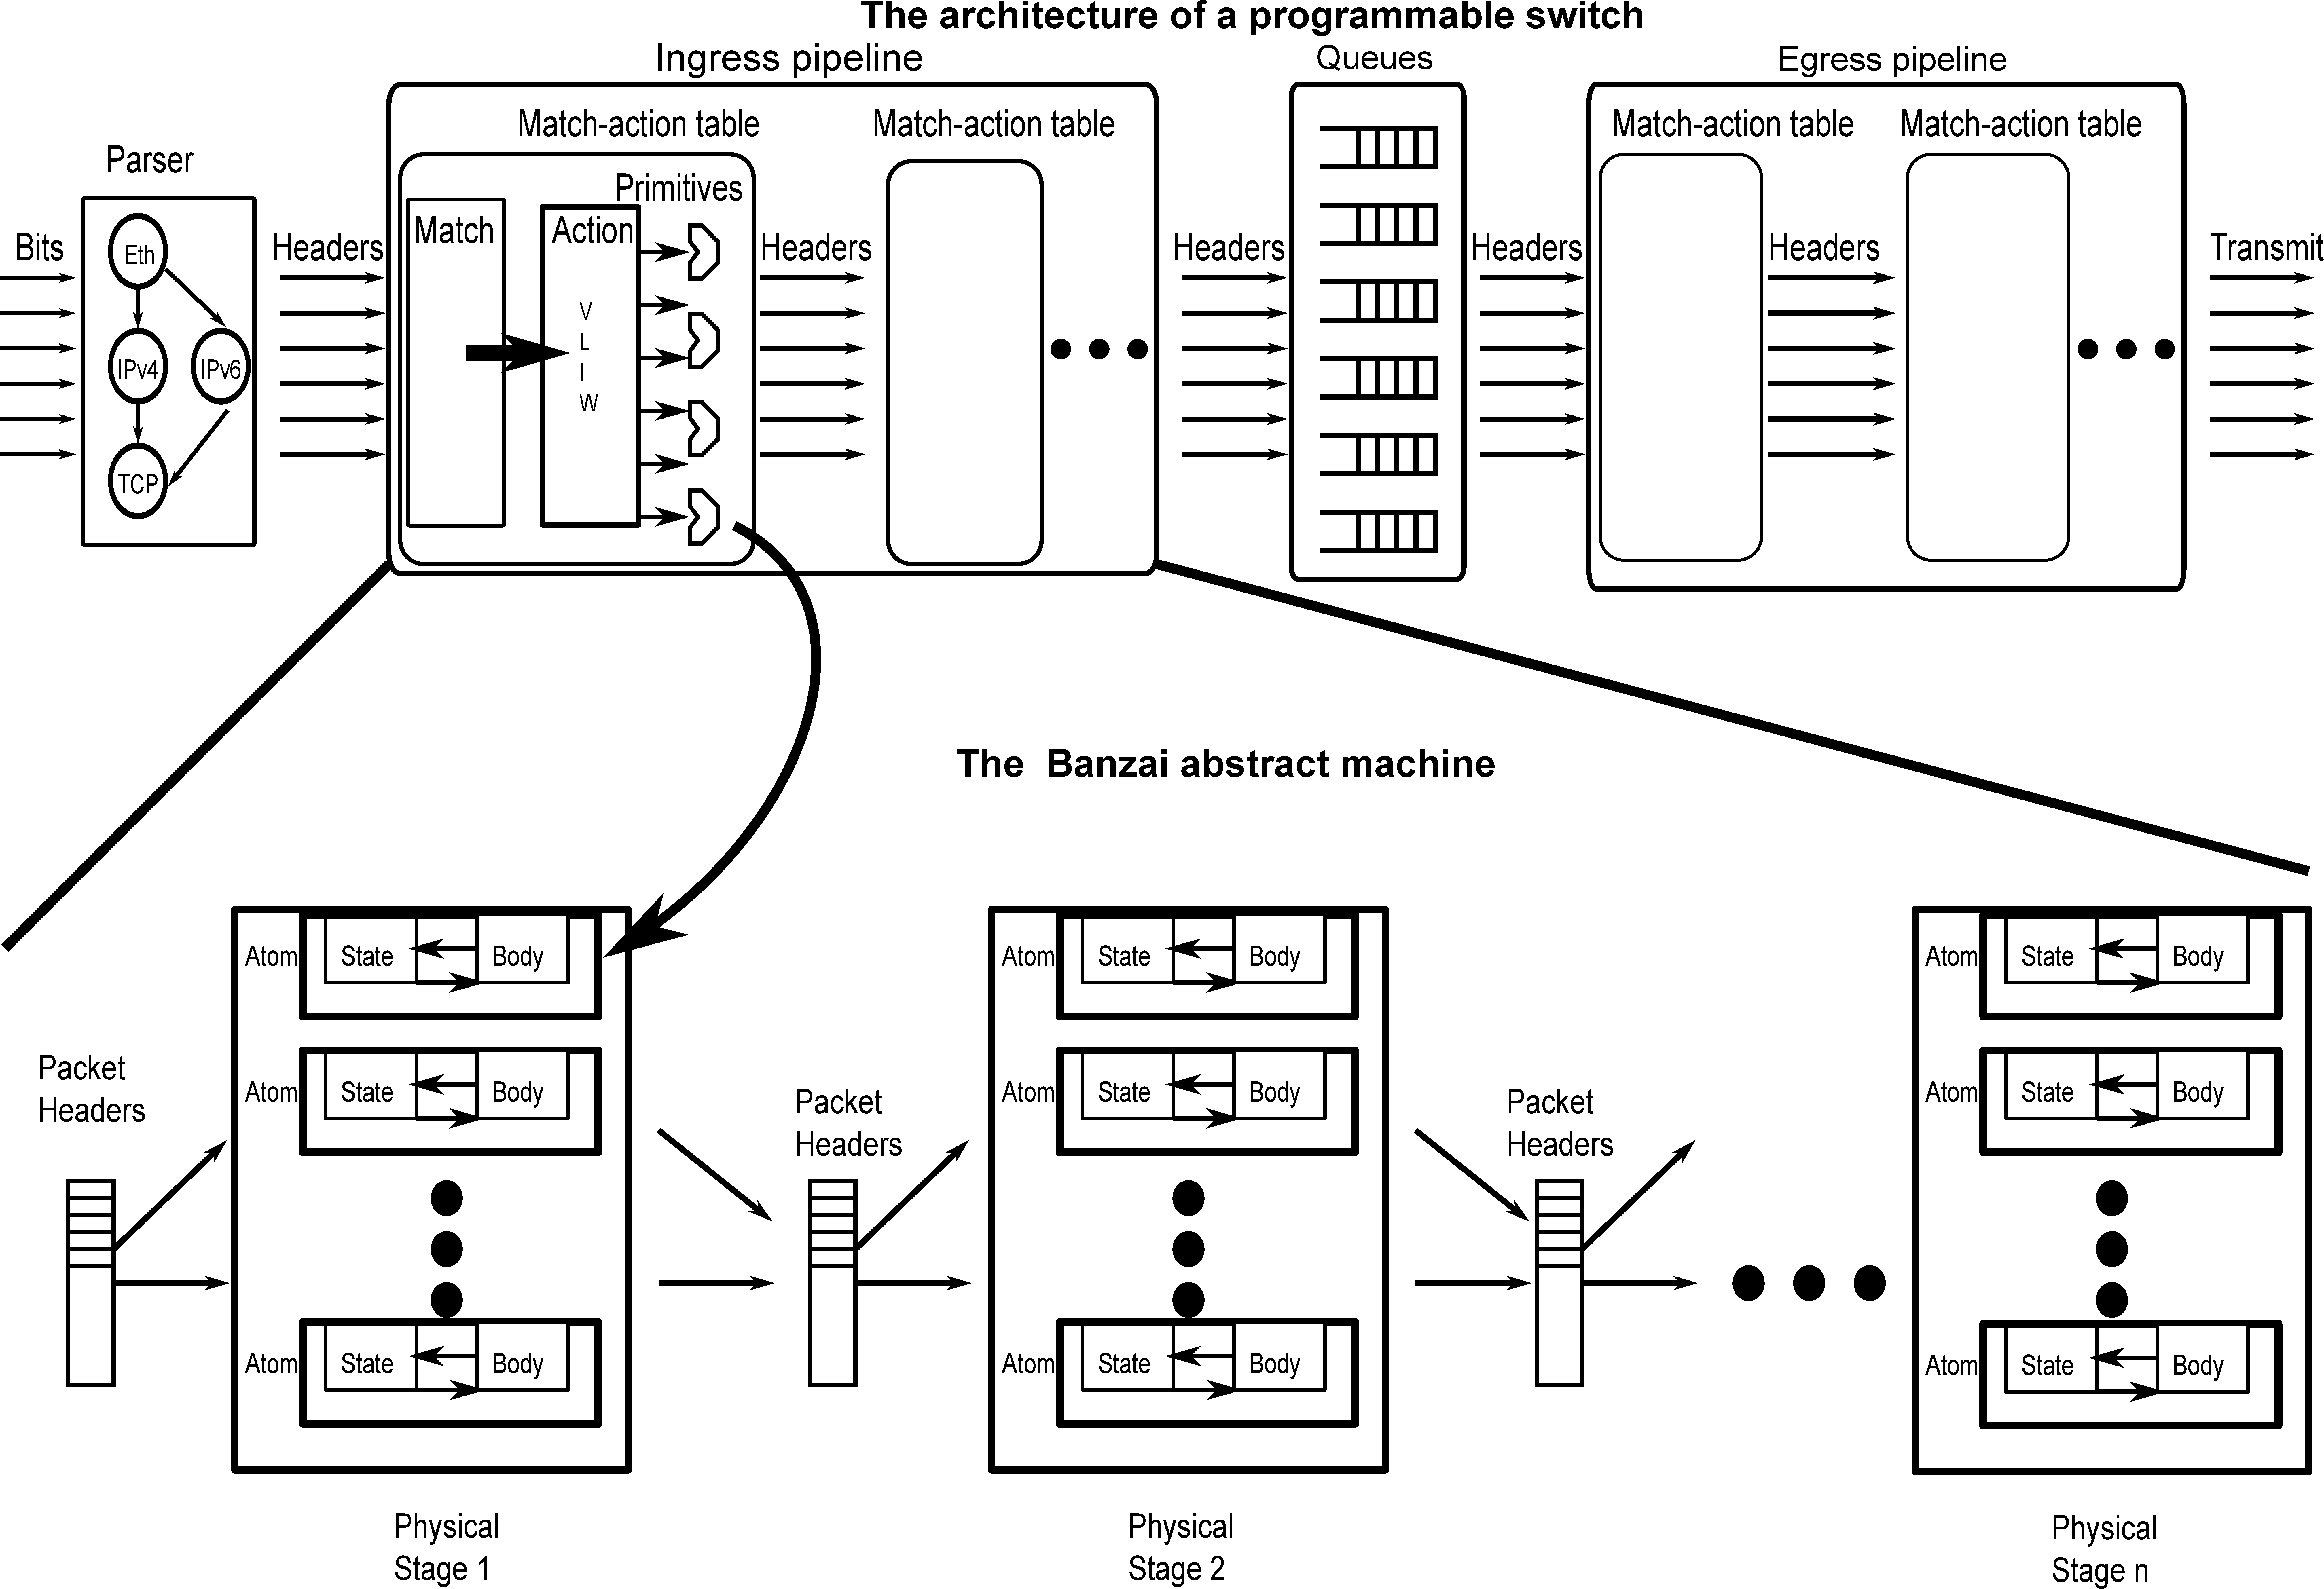
\includegraphics[width=\textwidth]{banzai.pdf}
  \caption{The \absmachine abstract machine and its relationship to programmable switch architectures.}
  \label{fig:switch}
\end{figure*}
Our abstract machine is directly inspired by programmable switch architectures
such as the Reconfigurable Match-Action Table architecture (RMT), Intel's
FlexPipe, and Cavium's XPliant. These architectures assume a switch model
(Figure~\ref{fig:switch}) that consists of an ingress pipeline, followed by the
switch scheduler, followed by an egress pipeline.

\absmachine is an abstract machine that models either of these two pipelines, with
the only difference being the packet fields available at the entrance of these
pipelines. Being an abstract machine, \absmachine only models mechanisms that are
critical to mapping data-plane algorithms. In particular, it models the
computation that happens in each match-action table (i.e. the action half of
the match-action table), but not the match semantics (direct, ternary, or longest
prefix). Notably, \absmachine doesn't model packet parsing.

A switch pipeline in \absmachine has a number of pipeline stages that execute
in parallel with a packet being handed off from one pipeline stage to the next.
Each stage contains a vector of \textit{atoms}, with the atoms themselves
executing in parallel. Informally, an atom is an atomic unit of packet
processing and is represented by a body of imperative code that executes
sequentially. An atom is assumed to complete execution and modify a packet
before the next packet is processed by that atom.

An atom may also contain internal state that can influence the atom's behavior
from one packet to the next and persists across packets. For instance, a switch
counter could be written as an atom as follows\footnote{We use the notation p.x
  to represent access to field ``x'' within a packet p and the notation x to
represent access to the state variable ``x'' that persists across packets}.
\begin{verbatim}
  p.tmp     = counter;
  p.tmp2    = p.tmp + 1;
  counter   = p.tmp2;
\end{verbatim}
Similarly, a stateless operation that sets a packet field, such as the
modify\_field action primitive in P4 (equivalently, the bitmasked-set operation
from the RMT architecture) can be written as the atom below:
\begin{verbatim}
  p.field   = value;
\end{verbatim}

The \absmachine abstract machine generalizes several aspects of a programmable
switch architecture. The vector of atoms in each stage generalizes RMT's
very-large instruction-word (VLIW)~\cite{rmt} that executes primitive actions
on independent packet fields in parallel. The presence of internal state in an
atom models persistent switch state residing on a switch such as meters,
counters, , and P4's register abstraction in a unified manner.

\textbf{Constraints on atoms} \\

Any switch hardware running at line rate will need to constrain atoms to bound
the execution latency of each atom and provide deterministic performance. We
impose two such constraints that distinguish \absmachine from software
packet-processing platforms such as Click and Network Processors such as the
Intel IXP, which tradeoff deterministic performance for greater flexibility in
expressing packet processing code.

First, \absmachine is a shared-nothing architecture: state variables are internal to
a particular atom and their values can only be communicated with atoms in
subsequent stages by writing these state variables into packet fields that are
then read downstream.  This restriction reflects the capabilities of most
switches today: building memories that can be simultaneously accessed from
multiple switch stages is technically challenging.

%%To let a stage communicate state information to a predecessor stage upstream,
%%\absmachine allows packets to be cloned and recirculated back into a pipeline,
%%modeling the loopback interfaces found on most switches today.
Second, we constrain the complexity of atom bodies by definining how atoms are
executed. One execution model is an in-order load-store CPU that can execute at
most $N$ instructions sequentially. Another is a configurable combinational
circuit in hardware~\cite{dataflow}, where the circuit limits the space of
feasible computations and needs its control signals to be configured to match
the behavior of the atom.

We use both models in this paper. For stateless atoms that don't modify state,
we constrain atom bodies to consist of only statements that can be represented
as three-instruction codes. Further, we allow exactly one statement in each
atom body. This corresponds to the set of primitive actions available today in
P4/RMT.  For atoms that do modify state, we consider both models
(\S\ref{s:constraints}) and evaluate how atom body constraints affect whether
or not packet-processing code can be mapped onto \absmachine.

% --> Packet transactions and how this is different from other transactions.
\subsection{Packet transactions}
\begin{figure}
  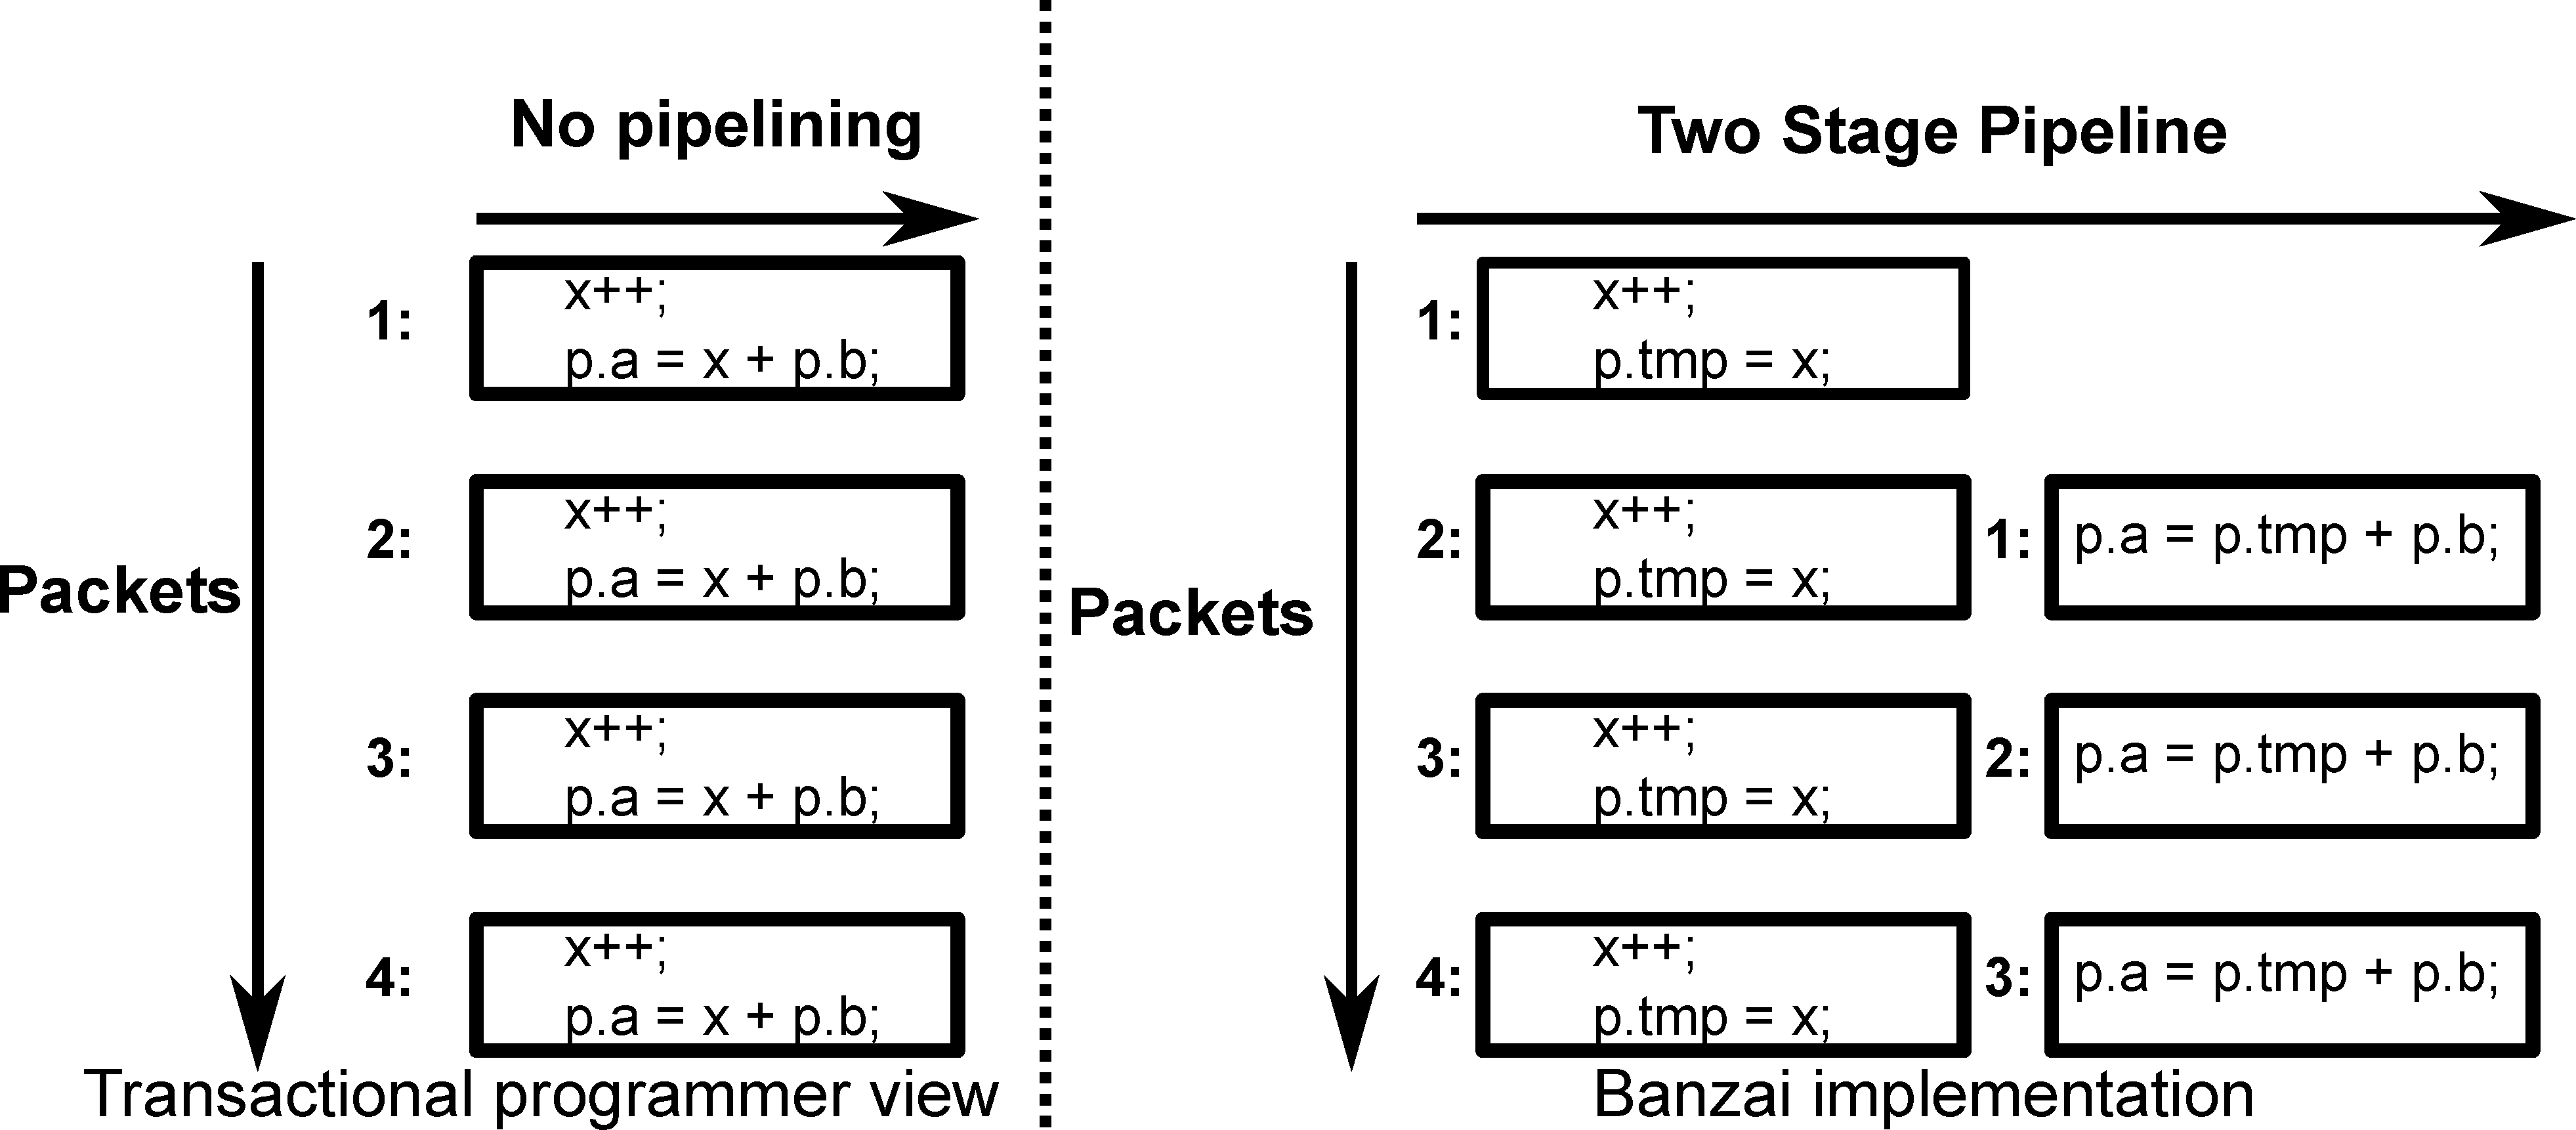
\includegraphics[width=\columnwidth]{spec_vs_impl.pdf}
  \caption{A packet transaction and its implementation}
  \label{fig:trans}
\end{figure}

Having described our target architecture, we now describe a programming model
for it, inspired by database transactions. Transactions are the strongest
guarantee that a database system can provide in that the effect of a
transaction is either entirely visible or not with no intermediate state being
visible to the outside world.

We repurpose database transactions for data-plane programming by defining the
notion of a \textit{packet transaction}: a body of sequential code that
executes from start to finish on each packet and conceptually processes only
one packet at a time. For a programmer, the packet transaction represents
exactly what happens to every packet. Every packet is processed in isolation
and to completion before the next packet's processing begins.

In practice though, switch hardware is heavily pipelined
(Figure~\ref{fig:switch}).  A compiler automatically translates the
programmer's transactional code block into a low-level pipelined implementation
on the switch hardware (Figure~\ref{fig:trans}).

Put differently, the user's packet transaction is a single atom that captures
all computations on the packet and encapsulates all the state required to carry
out the computation.  A compiler then translates this packet transaction into
into a grid of atoms that is functionally equivalent to the single atom, while
respecting hardware constraints on each atom's complexity. If the compiler is
unable to find a mapping, it rejects the packet transaction as being too
complex for the given target.

\section{A Language for data-plane algorithms}
\label{s:language}

As previously described, data-plane algorithms are characterized by an
irregular control flow and extensive use of stateful processing. Based on these
observations, this section proposes a language to express these algorithms.

To motivate a language for these algorithms, we first observe that any
data-plane algorithm can be expressed as a function that takes in a single
packet and a set of persistent state variables as input. This function then
runs to completion without interruption, modifying the packet and the
persistent state variables in the process. Further, conceptually, only one
packet is processed by this function at any given instant.

This view of data-plane algorithms suggests a natural way to structure them: as
transactions where a function specifies all the required state manipulation and
control flow required for packet processing. The use of transactions is
widespread in packet processing for software-router platforms. For instance,
Click's Element abstraction~\cite{kohler_thesis} specifies packet processing as
a method invocation that isn't pre-empted.  The Linux qdisc
subsystem~\cite{qdisc} exposes an enqueue and dequeue method that specific
algorithms can implement. Intel's IXP architecture for NPUs uses a construct
resembling transactions called a Packet-Processing Stage
(PPS)~\cite{intel_pldi} to express packet processing code.
% https://github.com/torvalds/linux/blob/master/net/sched/sch_codel.c#L256

Relative to these prior systems, our contribution is in observing that
transactions can be profitably used to express data-plane algorithms for
high-speed line-rate switches as well. Realizing this practically requires us
to design a language that expresses packet processing within the body of the
transaction. A good language would strike the right balance between ease of
expression and ease of implementation. Programmable hardware switches
---although a significant advance over their fixed-function counterparts---are
still very restricted in the processing that they do on every packet. This
restriction is required to remain competitive with fixed-function switches.

Based on these observations, we describe our language for packet processing
(Figure~\ref{fig:language}). Our language is a heavily constrained subset of C
that removes all iterative constructs (while, do-while, for, break, continue),
arrays, heaps, and memory allocation. State variables are represented as global
variables. We permit structures to represent packet processing alone, and immediately
desugar these to scalar variables (\S\ref{s:compiler}).

Forbidding loops and other sources of variable performance like memory
allocation, and array scans allows the user to only express code whose
execution latency can be bounded at compile time.  While this may seem overly
restrictive, this is required for the underlying architecture
(\S\ref{s:architecture}), which has deterministic performance regardless of the
traffic pattern or program being run. This results in a different set of
tradeoffs than what programmers are typically used to: a larger program does
not take longer to run. Instead, it may not run at all or might need to be
approximated until it can run (\S\ref{ss:approximation}).

\section{The \pktlanguage compiler}
\label{s:compiler}

\begin{figure*}[!t]
  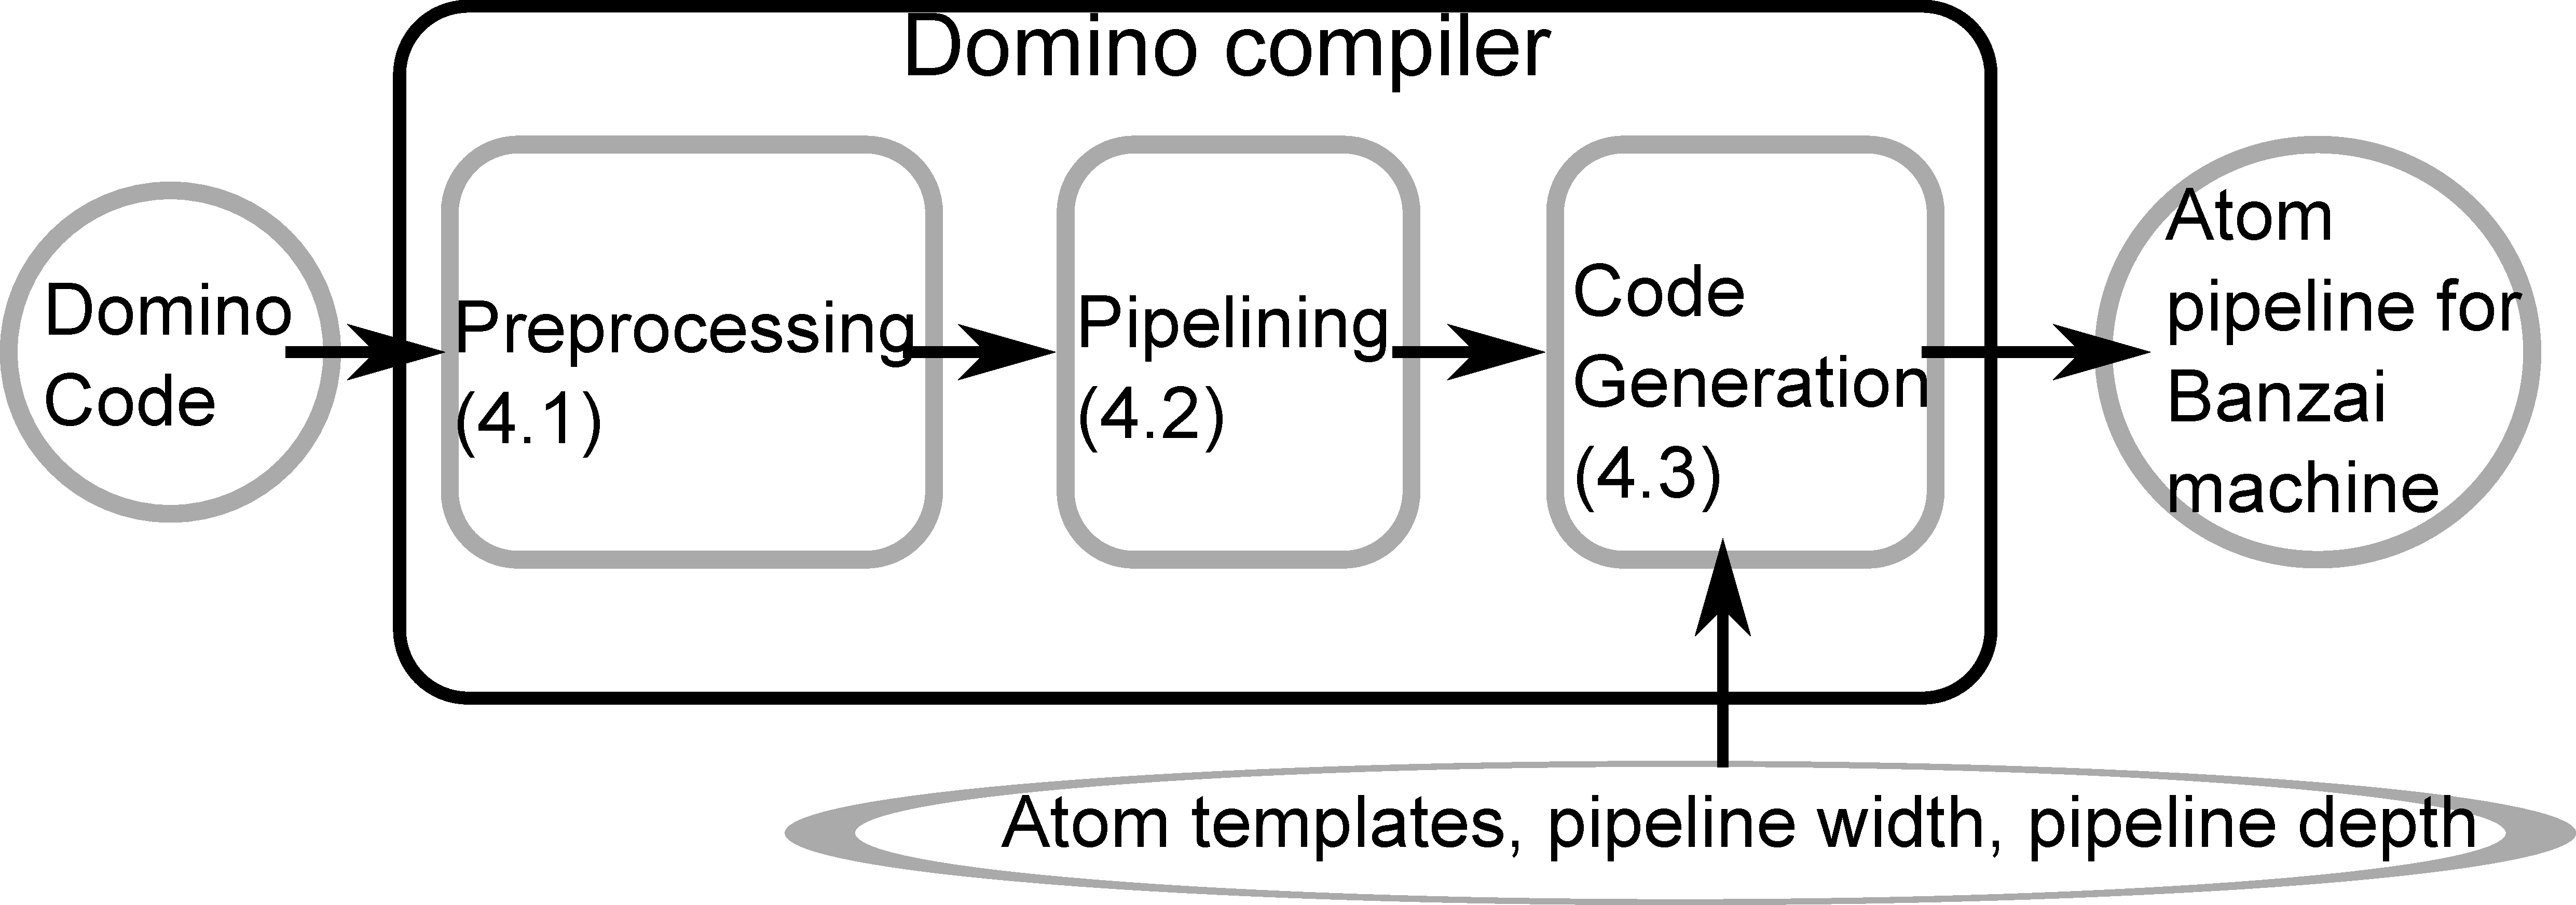
\includegraphics[width=\textwidth]{compiler.pdf}
  \caption{Passes in the \pktlanguage compiler}
\end{figure*}

The \pktlanguage compiler borrows several well-established techniques from the
compiler literature~\cite{muchnik}. However, as we show throughout this
section, constraining \pktlanguage for deterministic performance has a happy
side effect: it allows us to considerably simplify the \pktlanguage compiler
relative to mainstream compilers.

\subsection{Lexing, parsing, and semantic analysis}
Because \pktlanguage's syntax is based on C, we use clang's library
interface~\cite{libclang} to generate an Abstract Syntax Tree (AST) for packet
transactions written in \pktlanguage. The remaining compiler passes operate on
this AST. Basing \pktlanguage's syntax on C has several benefits.  Clang's
frontend catches several errors with no additional effort. It also
allows us to use the C macro preprocessor for constants. Intrinsic
functions representing hardware primitives (e.g.  hashes), can be
implemented using arbitrary C code and linked with \pktlanguage code before
running the resulting binary on a \absmachine machine.
%(\S\ref{ss:verification}).

\subsection{If-conversion to straight-line code}
A packet transaction's body can contain if-else statements that alter control
flow and complicate dependence analysis. We eliminate if-else statements by
transforming them into the C conditional operator, starting from the innermost
if statements and recursing outwards (Figure~\ref{fig:if_convert}). This
procedure is called if-conversion~\cite{if_conversion}; it is much simpler in
\pktlanguage because only if-else statements alter control flow in
\pktlanguage; all other control transfer (break, continue, loops) is forbidden.
This transformation creates straight-line code, where control passes
sequentially without branching. Straight-line code simplifies the rest of the
compiler, like computing the SSA(\S\ref{ss:ssa}).

\begin{figure*}[!t]
  \begin{minipage}{0.47\textwidth}
  \begin{small}
  \begin{lstlisting}[style=customc]
if (pkt.arrival -
    last_time[pkt.id] >
    THRESHOLD) {
 saved_hop[pkt.id] = pkt.new_hop;
}
  \end{lstlisting}
  \end{small}
  \end{minipage}
  \begin{minipage}{0.53\textwidth}
  \begin{small}
  \begin{lstlisting}[style=customc]
pkt.tmp = pkt.arrival -
          last_time[pkt.id]
          > THRESHOLD;
saved_hop[pkt.id] = pkt.tmp ?
                    pkt.new_hop :
                    saved_hop[pkt.id];
  \end{lstlisting}
  \end{small}
  \end{minipage}
\caption{Conversion to straight-line code}
\label{fig:if_convert}
\end{figure*}
\subsection{Converting state variables to load/store form}

We next identify state variables used in a packet transaction, both arrays and
scalars, such as \texttt{last\_time} and \texttt{saved\_hop} in
Figure~\ref{fig:flowlet}. For each state variable, we create a \textit{read
flank} to read the state variable into a temporary packet field. For an array,
we also move the index expression into the read flank, exploiting the fact that
only one array index is accessed by each packet in valid \pktlanguage
programs.  Then, we replace all occurrences of the state variable with the
packet temporary, and create a \textit{write flank} to write the packet
temporary back into the state variable.  Figure ~\ref{fig:stateful_flanks}
illustrates this transformation on a fragment.  After this pass, the code
resembles code for a load-store architecture~\cite{load_store}: state variables
only support reads and writes; arithmetic happens on packet variables.
Restricting the operations on state variables simplifies their treatment
during code partitioning (\S\ref{ss:partitioning}).


\begin{figure*}[!t]
  \begin{minipage}{0.47\textwidth}
  \begin{small}
  \begin{lstlisting}[style=customc]
pkt.id = hash2(pkt.sport,
               pkt.dport)
         % NUM_FLOWLETS;
last_time[pkt.id] = pkt.arrival;
  \end{lstlisting}
  \end{small}
  \end{minipage}
  \begin{minipage}{0.53\textwidth}
  \begin{small}
  \begin{lstlisting}[style=customc]
// Read flank for last_time
pkt.id = hash2(pkt.sport,
                pkt.dport)
         % NUM_FLOWLETS;
pkt.last_time = last_time[pkt.id];

pkt.last_time = pkt.arrival;

// Write flank for last_time
last_time[pkt.id] = pkt.last_time;
  \end{lstlisting}
  \end{small}
  \end{minipage}
  \caption{Adding read and write flanks}
\label{fig:stateful_flanks}
\end{figure*}

\subsection{Renaming variables to static single-Assignment Form}
\label{ss:ssa}

We next convert to static single-assignment form (SSA)~\cite{ssa}, an
intermediate form used by many compilers~\cite{tree_ssa, llvm}.  In SSA, every
variable is assigned exactly once. To compute the SSA, we replace every
definition of a packet variable with a new packet variable and propagate this
new packet variable until the next definition of the same variable. State
variables are already in SSA form: after their flanks have been added, every
state variable is written exactly once in the write flank.  While general
algorithms for computing the SSA are fairly involved~\cite{ssa}, \pktlanguage's
SSA computation is simpler because it operates on straight-line code.  SSA
simplifies further analysis. Every variable is assigned exactly once, implying
that there are no Write-After-Read or Write-After-Write dependencies. Only
Read-After-Write dependencies remain, simplifying dependency
analysis during code partitioning (\S\ref{ss:partitioning}).

\begin{figure*}[!t]
  \begin{minipage}{0.48\textwidth}
  \begin{small}
  \begin{lstlisting}[style=customc]
pkt.id = hash2(pkt.sport,
               pkt.dport)
               % NUM_FLOWLETS;
pkt.last_time = last_time[pkt.id];
pkt.last_time = pkt.arrival;
last_time[pkt.id] = pkt.last_time;
  \end{lstlisting}
  \end{small}
  \end{minipage}
  \begin{minipage}{0.52\textwidth}
  \begin{small}
  \begin{lstlisting}[style=customc]
pkt.id0 = hash2(pkt.sport,
                pkt.dport)
                % NUM_FLOWLETS;
pkt.last_time0 = last_time[pkt.id0];
pkt.last_time1 = pkt.arrival;
last_time[pkt.id0] = pkt.last_time1;
  \end{lstlisting}
  \end{small}
  \end{minipage}
  \caption{SSA transformation}
\label{fig:ssa}
\end{figure*}

\begin{figure*}[!t]
\begin{lstlisting}[style=customc]
pkt.id            = hash2(pkt.sport, pkt.dport) % NUM_FLOWLETS;
pkt.saved_hop     = saved_hop[pkt.id]; @\label{line:stateRead}@
pkt.last_time     = last_time[pkt.id];
pkt.new_hop       = hash3(pkt.sport, pkt.dport, pkt.arrival) % NUM_HOPS;
pkt.tmp           = pkt.arrival - pkt.last_time;
pkt.tmp2          = pkt.tmp > THRESHOLD;
pkt.next_hop      = pkt.tmp2 ? pkt.new_hop : pkt.saved_hop;
saved_hop[pkt.id] = pkt.tmp2 ? pkt.new_hop : pkt.saved_hop; @\label{line:stateWrite}@
last_time[pkt.id] = pkt.arrival;
\end{lstlisting}
\caption{Flowlet switching in three-address code}
\label{fig:three_address}
\end{figure*}

\subsection{Expression flattening to three-address code}
We next transform into three-address code~\cite{tac}, where all instructions
are either reads / writes into stateful variables or carry out packet
manipulations of the form: \texttt{pkt.f1 = pkt.f2 op pkt.f3;} where
\texttt{op} includes all arithmetic, logical, and relational operators. We also
allow either pkt.f2 or pkt.f3 to be an intrinsic function call, because we
assume these are supported in hardware. To generate three-address code, we
flatten expressions that are not already legal in three-address code, by
introducing enough temporaries
(Figure~\ref{fig:three_address}).
%Three-address code instructions are similar to P4's action
%primitives~\cite{p4spec} and RMT's VLIW instruction set~\cite{rmt}. 

\subsection{Code partitioning to codelets}
\label{ss:partitioning}
At this point, the code is still sequential. Code partitioning turns sequential
code into a pipeline of \textit{codelets}, where each codelet is a small
sequential block of three-address code statements. We generate this pipeline of
codelets, by exploiting parallelism within and across pipeline stages.
Subsequently, we map each codelets one-to-one to atoms provided by a particular
\absmachine machine~(\S\ref{ss:code_gen}), returning a compiler error if any
codelet doesn't map to an atom provided by the hardware.

To partition code into codelets, we carry out the following steps:
\begin{CompactEnumerate}
  \item Create a node for each statement (Figure~\ref{fig:three_address}) in
    the packet transaction after expression flattening.
  \item Create a bidirectional edge between N1 and N2 where N1 is a read from a
    state scalar / state array and N2 is a write into the same state scalar /
    state array. This step captures the constraint that state is internal to an
    atom in \absmachine. Because state variables don't occur in any
    instructions besides reads and writes, this is all we need to do to handle
    state variables.
  \item Create an edge (N1, N2) for every pair of nodes N1, N2 where N2 reads
    a variable written by N1. We only check read-after-write dependencies because
    control dependencies turn into data dependencies when generating straight-line
    code. Further, the use of SSA removes all write-after-read and write-after-write
    dependencies.
  \item Generate strongly connected components (SCCs) of the resulting graph
    (Figure~\ref{fig:partitioning}a) and condense the SCCs to to create a directed
    acyclic graph (DAG) (Figure~\ref{fig:partitioning}b). This step captures the
    constraint that all operations on state variables (read, write, and modify)
    must reside within the same atom because state is local to an atom.
  \item Schedule the resulting DAG using critical path
    scheduling~\cite{crit_path_sched}, creating a new pipeline stage every time
    one operation needs to follow another (Figure~\ref{fig:flowlet}b).
\end{CompactEnumerate}
At this point, the resulting codelet pipeline (Figure~\ref{fig:flowlet}b)
implements the packet transaction.  Further, the codelets themselves have a
stylized form.  Codelets that don't manipulate state contain exactly one
three-address code instruction. Codelets that manipulate state contain at least
two statements: a read from a state variable and a write to a state variable
and optionally consist of one or more updates to the state variable through
packet temporaries.

\begin{figure*}[!t]
\begin{minipage}{0.5\textwidth}
  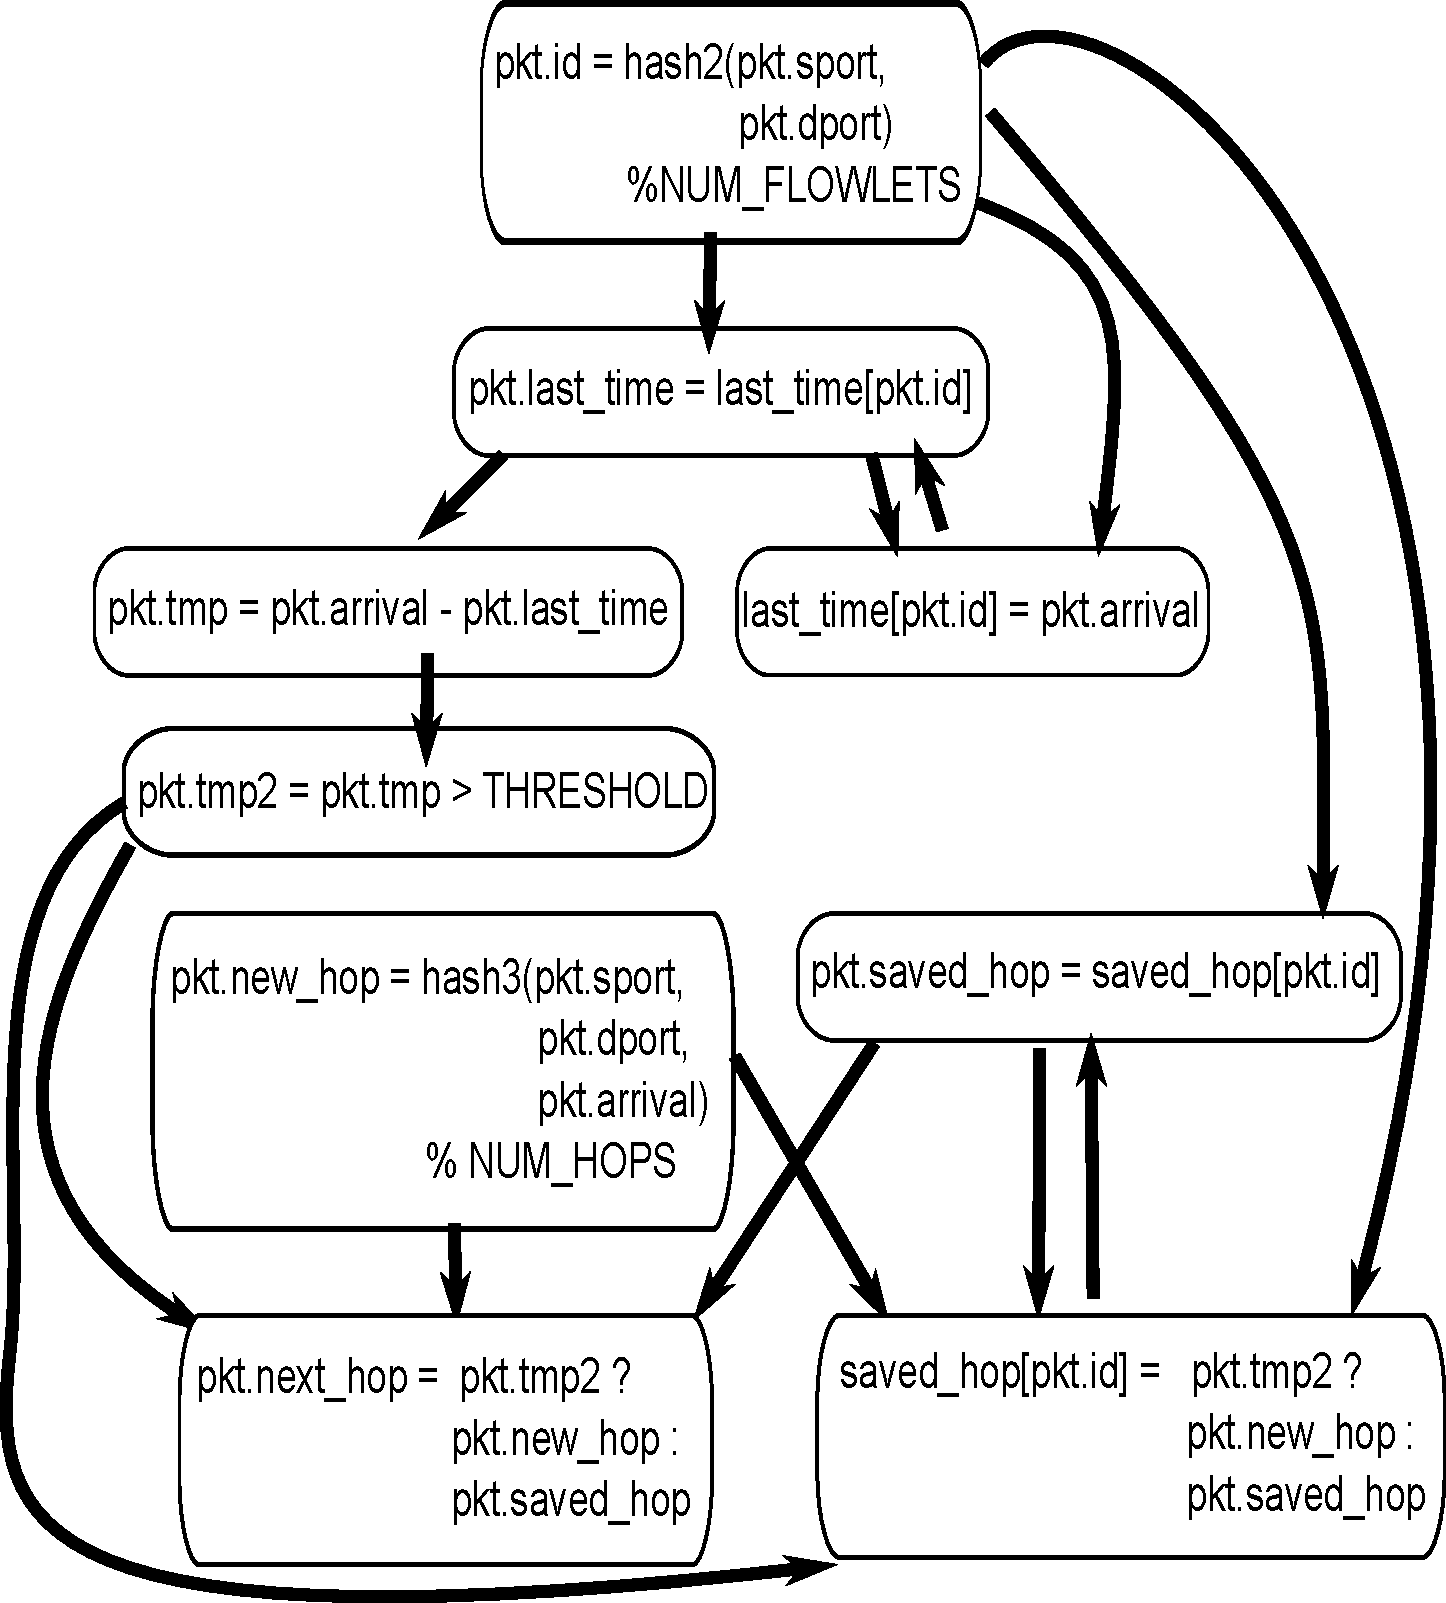
\includegraphics[width=\columnwidth]{deps.pdf}
\end{minipage}
%
\vrule\quad
%
\begin{minipage}{0.5\textwidth}
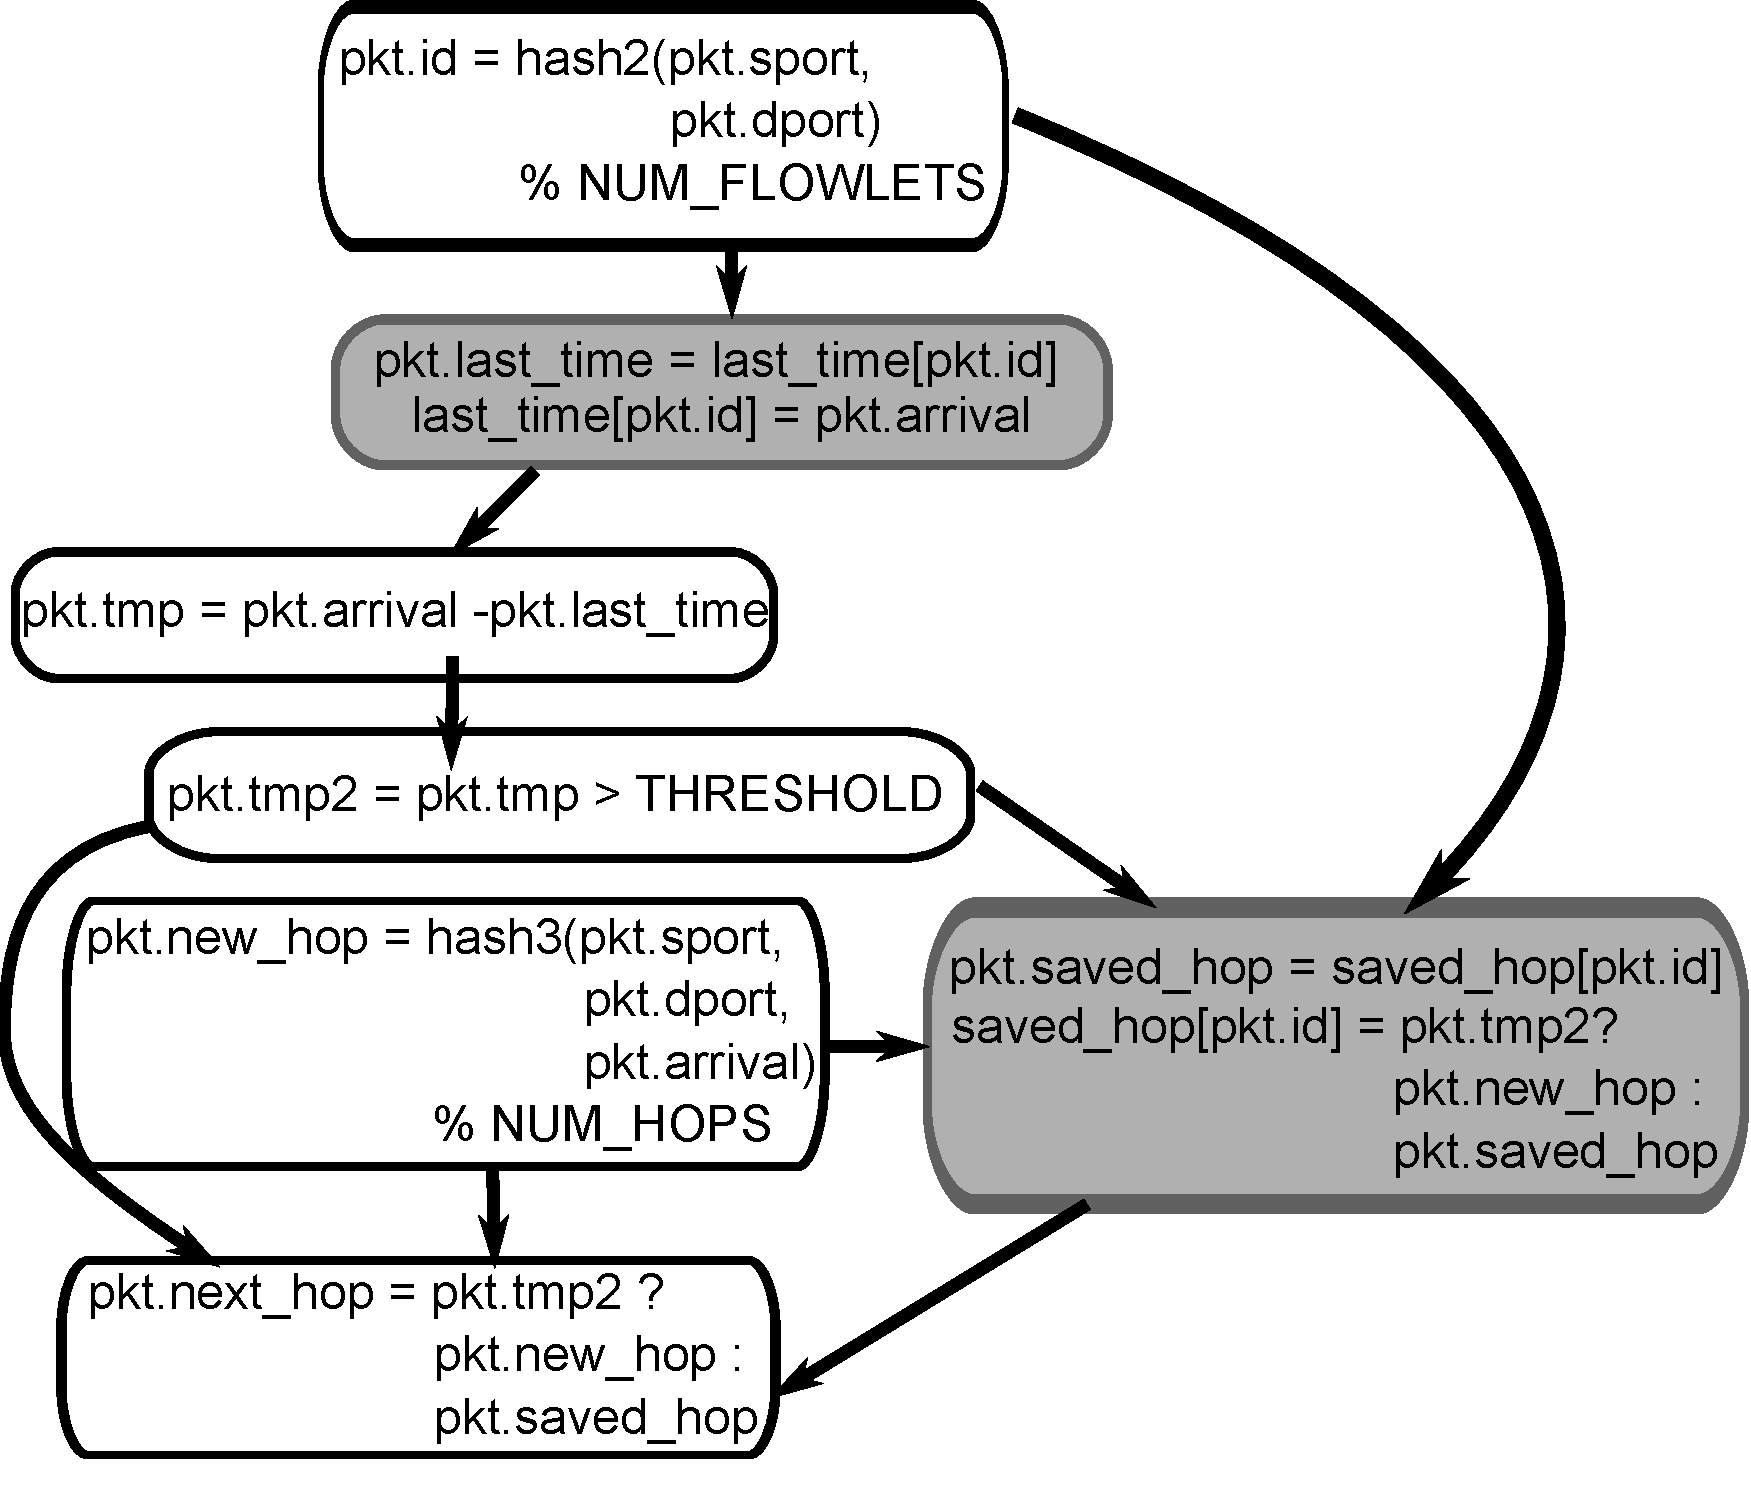
\includegraphics[width=\columnwidth]{scc.pdf}
\end{minipage}
\caption{Dependency graph (a) before and (b) after condensing strongly connected components}
\label{fig:partitioning}
\end{figure*}

\subsection{Code generation: Mapping a codelet to an atom}
\label{ss:code_gen}
Next, we determine how the codelets created by code partitioning in the
previous step map one-to-one to atoms provided by the \absmachine machine. We
consider codelets that do and don't manipulate state separately because we
handle each differently.

\textbf{Stateless codelets}
Expression flattening generates stateless codelets that each have only one
instruction in three-address code form (e.g. any of the unshaded boxes in
Figure~\ref{fig:flowlet}b). For this paper, we assume that all \absmachine
machines support all atoms that correspond to a single statement in
three-address code form. This assumption is backed by the fact that P4's
primitives~\cite{p4spec} and RMT's VLIW action set~\cite{rmt} both contain
instructions that are in three-address code form. With this assumption, mapping
a stateless codelet to an atom is trivial: each stateless codelet produced by
code partitioning has exactly one three-address code instruction, which is
equivalent to an atom available in the \absmachine machine. If the \absmachine
machine supports complex atoms beyond three-address code instructions, this
approach is still correct, although suboptimal. For instance, if the
\absmachine machine supports a multiply-and-accumulate atom~\cite{mac},
expression flattening would generate two atoms (one each for the multiply and
accumulate), where one suffices.

\textbf{Stateful codelets}
Stateful codelets have multi-line bodies that need to execute atomically. For
instance, updating the state variable \texttt{saved\_hop} in
Figure~\ref{fig:flowlet}b requires a read, followed by a conditional write.  It
is not readily apparent whether these codelets can be mapped to an available
atom. We develop a general technique to determine the implementability of such
stateful codelets, given as input the stateful atom template provided by the
\absmachine machine.

An atom template defines a space of possible computations (such as different
ALU operations, or different permitted sequences of $N$ three-address
instructions).  The exact computation is selected by \textit{configuring} the
atom. The codelet is a specification that is to be checked for functional
equivalence against one of the atom configurations supported by the atom
template. In other words, we need to \textit{synthesize} the atom's
\textit{configuration}, given an \textit{atom template} describing the atom's
functionality.

This is the realm of syntax-guided program synthesis~\cite{sgsyn}, where the
programmer supplies a partial program or template (hence the term
syntax-guided) with missing details, and a specification. A \textit{program synthesis
tool} then synthesizes these details in the partial program to ensure it matches
up bit exactly with the specification. One such program synthesis tool is
SKETCH~\cite{bitstreaming, sketch_asplos, sketch_manual}, which allows the
programmer to specify a partial program with \textit{holes} that are then
``filled in'' by SKETCH to match the specification
(Figure~\ref{fig:sketch}).

\begin{figure}[!b]
  \begin{center}
  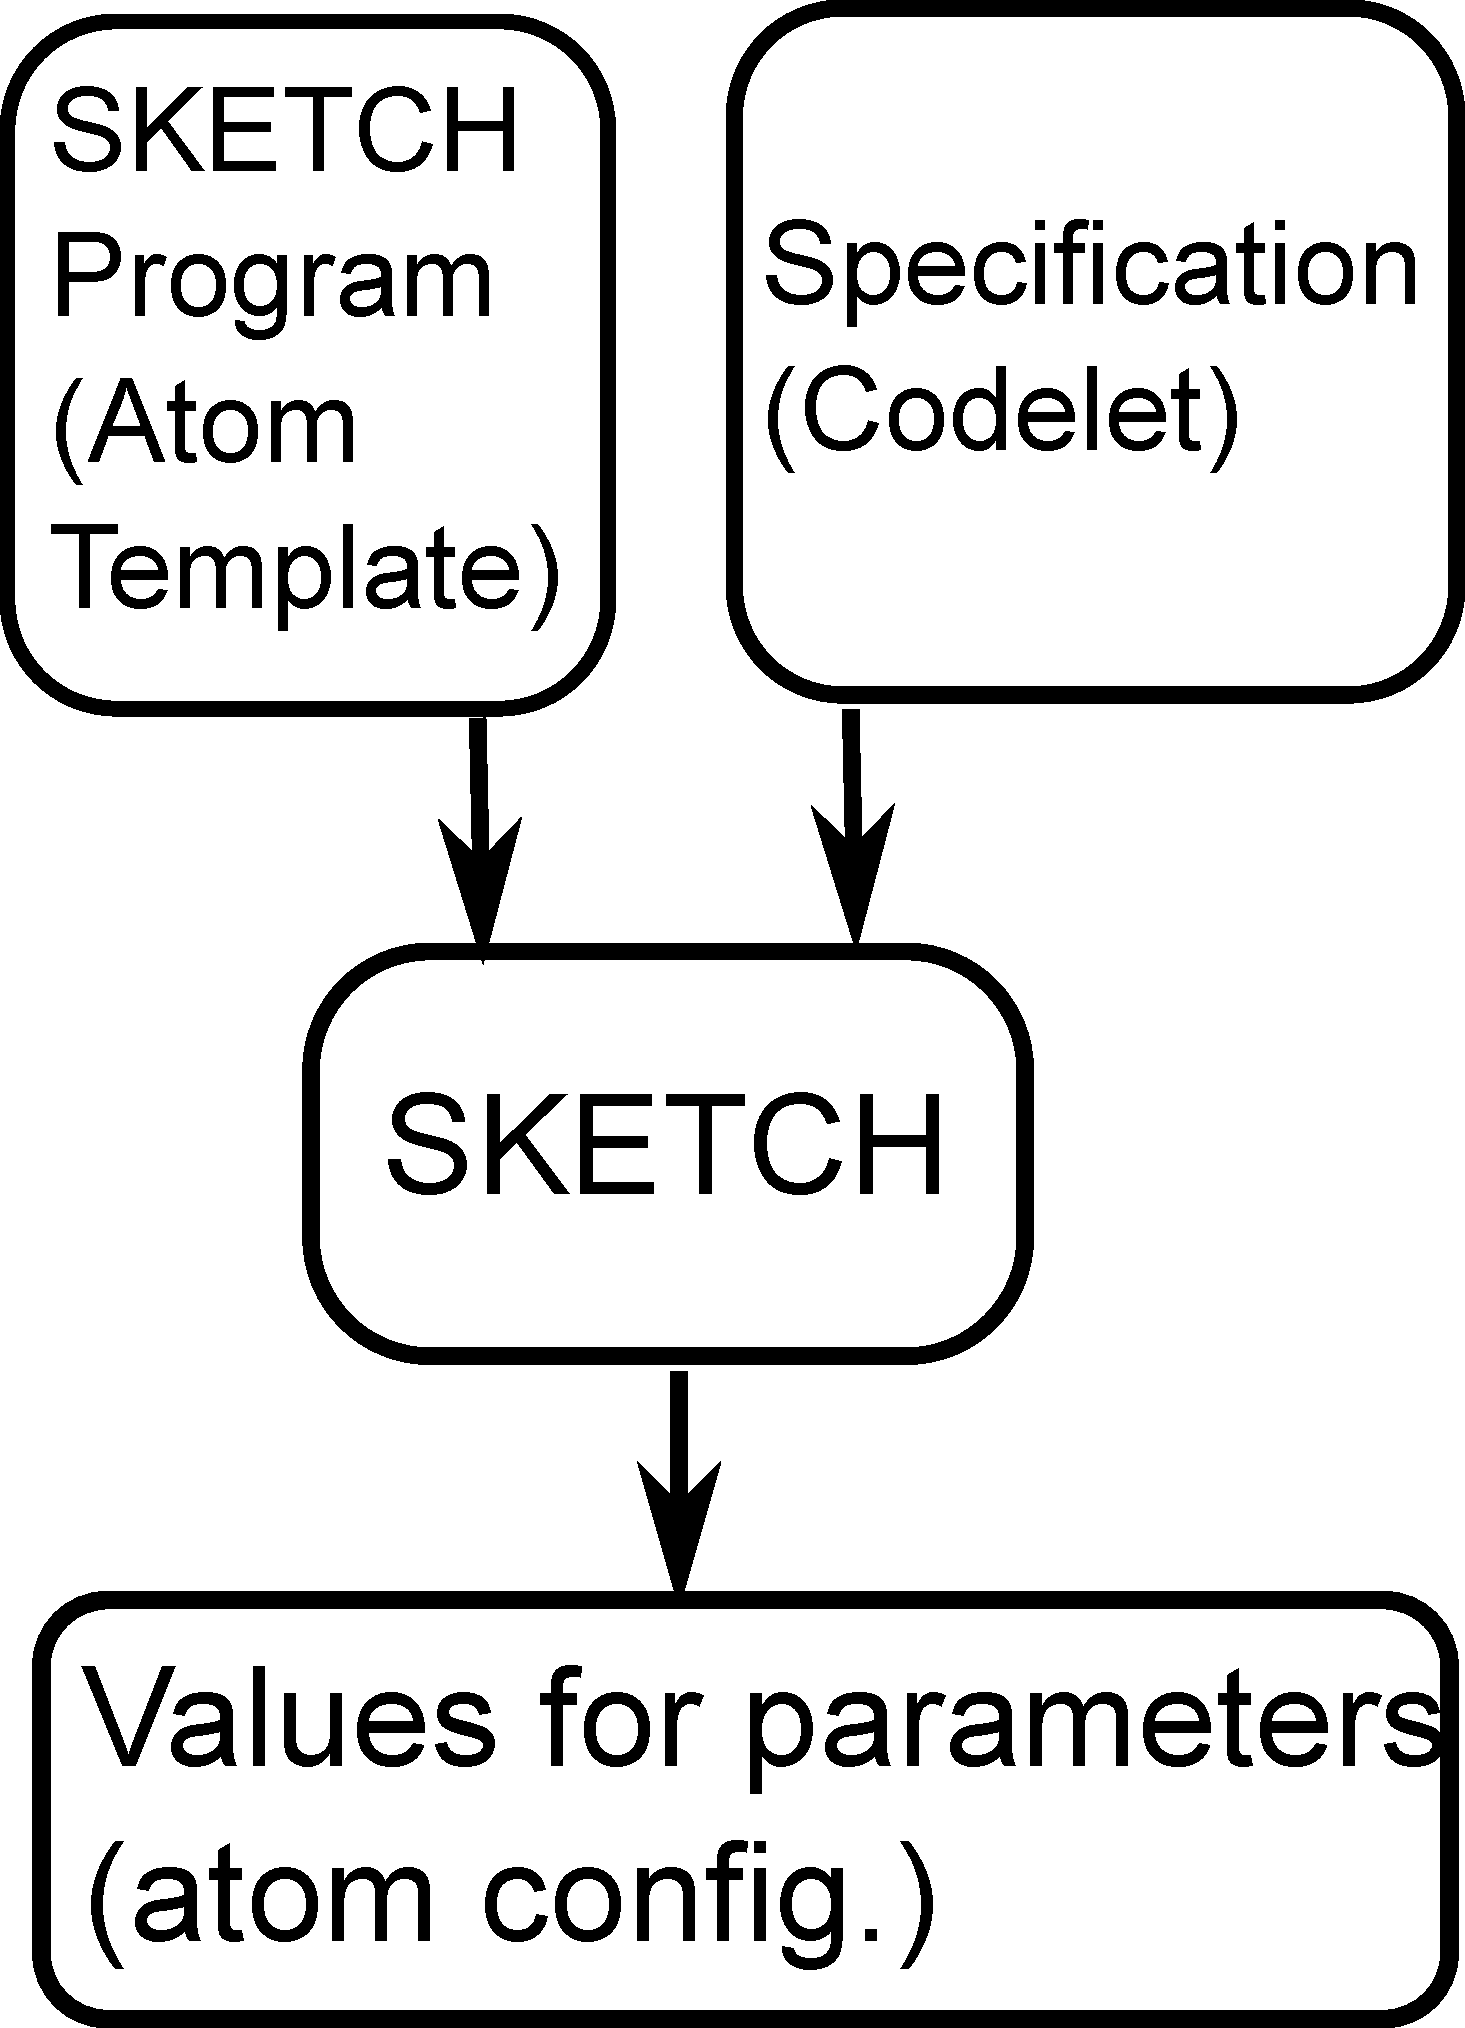
\includegraphics[width=0.4\columnwidth]{sketch.pdf}
  \caption{Overview of SKETCH and its application to atom configuration}
  \label{fig:sketch}
  \end{center}
\end{figure}

\begin{figure}[h]
  \begin{minipage}{0.4\columnwidth}
  \begin{center}
  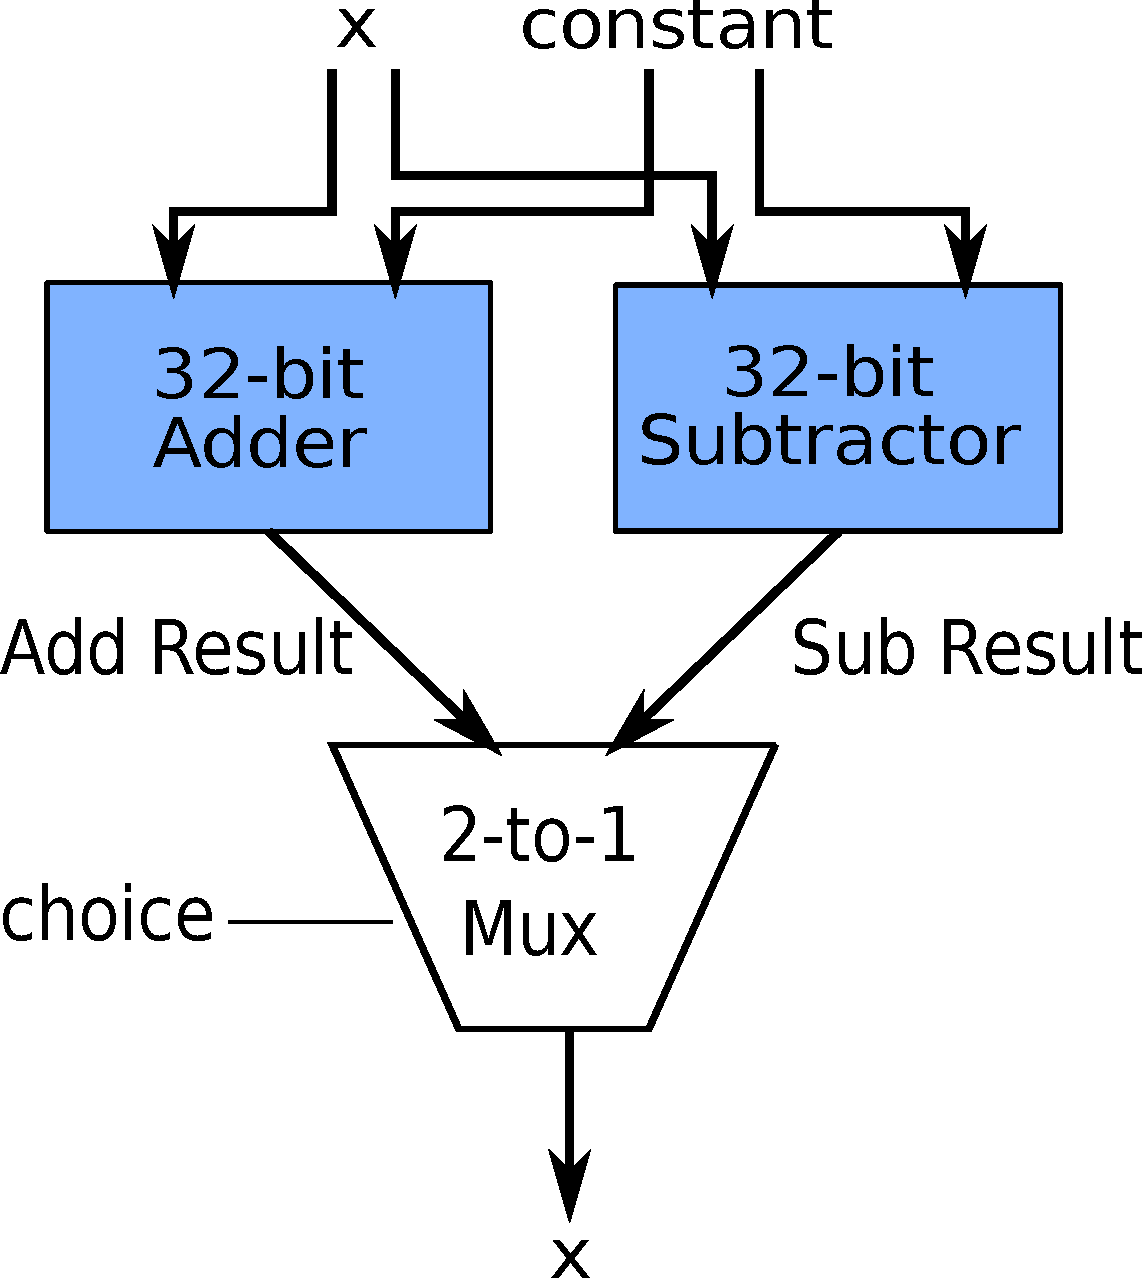
\includegraphics[width=\columnwidth]{circuit.pdf}
  \end{center}
  \end{minipage}
  \begin{minipage}{0.55\columnwidth}
  \begin{center}
  \begin{lstlisting}
  bit choice = ??(1);
  int constant = ??(16);
  if (bit) {
    x = x + constant;
  } else {
    x = x - constant;
  }
  \end{lstlisting}
  \end{center}
  \end{minipage}
\caption{\small (a) Circuit for an atom that can either add or subtract a
constant from a state variable.  (b) Circuit's representation in SKETCH.
Each ``??(n)'' represents a hole that can be filled in with values in
  $[0, 2^n -1]$.}
\label{fig:alu_in_sketch}
\end{figure}

We use SKETCH to solve the atom configuration problem.  Consider an atom
template that models an ALU (Figure~\ref{fig:alu_in_sketch}a) taking two
configuration parameters: an opcode, \texttt{choice}, specifying an addition or subtraction
operation, and a 16-bit positive constant, \texttt{constant}.  The ALU's functionality is to add
or subtract this constant from one state variable. This ALU can be represented
by the SKETCH partial program given in Figure~\ref{fig:alu_in_sketch}b.

Let's say we want to map the codelet x=x+1 to this atom. The codelet is then
fed into SKETCH as the desired specification and the atom template is fed into
SKETCH as the partial program (Figure~\ref{fig:sketch}). SKETCH will configure
the atom template by setting \texttt{choice} to 0 and \texttt{constant} to 1.
On the other hand, if the codelet x = x * x was supplied as the specification,
SKETCH will return an error because the specification cannot be mapped to any
of the computations provided by the atom template. We don't describe the
algorithms underlying SKETCH because we treat SKETCH as a blackbox in the
\pktlanguage compiler. The interested reader is referred to~\cite{bitstreaming,
sketch_asplos} for a more detailed treatment of these topics.

Using SKETCH to represent atom templates allows us to express the behavior of
diverse atoms (Table~\ref{tab:templates}) using a natural imperative syntax.
Because different \absmachine machines only differ in the atoms they provide,
employing SKETCH for atom configuration lets us build a retargetable
compiler~\cite{lcc} with little target-dependent work beyond specifying each
target's atoms as partial programs in SKETCH.

\subsection{Verifying compilations}
\label{ss:verification}

To conclude, we describe our testing infrastructure to verify that the
compilation is correct i.e. the externally visible behavior of the packet
transaction (Figure~\ref{fig:flowlet}a) is indistinguishable from its pipelined
implementation (Figure~\ref{fig:flowlet}b). We verify correctness by feeding in
the same set of test packets to both the packet transaction and its
implementation and comparing the outputs from both programs on the set of
externally visible fields. To create test packets, we scan the packet
transaction and generate the set of all packet fields read from or written to
by the transaction. We then initialize each of these fields by sampling
independently and uniformly from the space of all 32-bit signed integers.

% TODO: Mihai thought I could shrink this.
To compare outputs from the packet transaction and its implementation, we track
renames that occur because of SSA. We compare each output field in the
transactional form with the last rename of the same output field in the
implementation. We then feed the same number of test packets to both the
specification and implementation and compare outputs at the end of the
pipeline. This allows to quickly ``spot check'' our compilations and
helped discover a few compiler bugs during development.

\input{testing}
\input{constraints}
\input{targets}
\section{Related work}
\label{s:related}
NPUs: Tradeoffs are different here. Each stage can do very very little on a switch relative to an NPU. NPUs are Turing-complete; here, on a switch, programs either fit or don't. If they don't fit, you need to approximate.

P4 compiler (Lavanya's work): Complementary backend.

CMU work on pipelining datapaths: Verilog and circuits.

P4 itself: Too low level. NetASM: Once P4 needs an IR, NetASM might be a good choice.

Click: P4 paper wrote it off. We think its worth revisiting here.

Fastpass or Flexplane: Say that you love the abstraction they propose,
but would love to do it at higher line rates.

Click, Maple, Flexplane: Proposed transactions first. We are inspired by them.

\section{Conclusion and Future work}
\label{s:future}
%\ac{What is the story about multiple transactions?}
% We are ditching that for now. Let's move it to future work.


% Multiple transactions
% We don't seem to be discussing types anywhere. We have only ints right now.
% Disclaim that somewhere.

% Can we come up with a hierarchy similar to Herlihy's hierarchy from his
% paper: Wait-Free synchronization?

% Future work:
%
%
% Front-end Optimizations,
% backtracking,
% type systems,
% tables,
% backend: register allocation + placement,
% approximations,
% formally proving correctness, and so on.
% Shared memory.
% I think the most interesting usability problem is providing useful
% diagnostics when things go wrong in the program and the compiler can't
% map the program. Basically, don't want to suffer the same fate as C++ templates.
% What if you could recirculate packets using a loopback interface?

% This snippet below is for when targets support sequenced instructions
%%% If the abstract machine supports more sophisticated instructions that are
%%% equivalent to combinations of two or more three-address instructions, e.g.  the
%%% multiply accumulate instruction (a*b + c), we imagine implementing instruction
%%% selection using tree tiling~\cite{inst_sel}.

\label{s:future}

In this paper we presented \pktlanguage, a new high-level language for expressing 
data-plane
algorithms. While our compiler prototype has achieved promising initial results, 
the design of our language opens up 
a number of interesting open problems to be explored:

\paragraph{Scheduling algorithms}
Packet scheduling~\cite{XXX, XXX} is another important class of data-plane algorithms.
However, they do not currently fit the \pktlanguage packet function abstraction
as scheduling decisions are often based on groups of packets rather than individual
ones. We will extend \pktlanguage, for instance by providing another class of packet
function that takes in a packet buffer as input, for implementing scheduling algorithms.
However, this will raise new challenges in compilation as packet buffers cannot be
easily implemented in our current backend (P4) \ac{check if true}.
\ac{any other classes besides scheduling?}

\paragraph{Richer program constructs}
Likewise, we will extend \pktlanguage to provide additional program constructs
to increase the expressivity of the language. For instance, supporting 
arrays and user-defined types. Such constructs are useful for expressing 
algorithms such as XXX and XXX.

\ac{drop this if not enough space}
\paragraph{Additional backends}
We will investigate compiling \pktlanguage to other backends in addition to P4. 
As a high-level language, \pktlanguage can be targeted to different backends, 
such as XXX, and even directly 
to switch hardware itself. \ac{is there a name for this? I suppose
it's not Verilog or VHDL} The goal is to implement different parts of the source 
program using different backends to leverage the benefits provided by each one:
\ac{give examples}.


\paragraph{Cost Modeling and Systematic Approximation}
As described in Section~\ref{s:context}, 
packet recirculation mechanism can be used to pass stateful variable values  
from a given stage to its predecessor,
in cases where the partitioner fails to combine such
operations into a single stage.
However, doing so results in approximating the semantics of
the input \pktlanguage program, as packets that are already in the pipeline 
while recirculation takes place might be processed based on stale values of the
switch. We will investigate analytical methods to quantify the effects of
such approximation on program semantics by leveraging recent work from
the programming languages community~\cite{sampsonApprox, chisel}. 
Furthermore, we will design cost
models to evaluate different partitionings and incorporate such methods into
the cost model as well. 


\if 0
1. Arrays and other aggregates.
2. Table layout: compiling to P4 and then go down. Make it the P4 compiler's problem.
TCP traffic and end-to-end evaluation of approximation quality like video quality in approximate computing.
So far our approach to evaluating approximations is empirical, not analytical. Analysis would be awesome.
3. Scheduling, by definition, requires looking at multiple packets together to
make a decision on what packet to schedule next, while data-plane algorithms
operate independenly on each packe
\fi


{\footnotesize \bibliographystyle{acm}
\bibliography{paper}}

\end{document}
